\documentclass{article}
\title{CSCI 2200 HW1}
\author{Xinshi,Wang}
\usepackage[letterpaper,textwidth=5.5in,right=0.6in,textheight=9in,left=0.6in,top=0.7in,bottom=0.7in]{geometry}
\usepackage{scrextend}
\usepackage{graphicx}
\usepackage{xcolor}
\usepackage{amssymb}
\usepackage{amsmath}
\usepackage{setspace}
\usepackage{mathrsfs}
\usepackage[utf8]{inputenc}
\usepackage{mathtools}
\begin{document}
\noindent
CSCI 2200 HW1\\
Wang Xinshi\\

%Q (1.21) starts from here
\noindent Q 25.8(f) Find the CFG for Strings with more 0s than 1s.
\\\\
If there are more 0s than 1s, we can construct a CFG that when producing 1s it must produces 2 0s.\\
\begin{align}
	S \rightarrow &\epsilon \\
	S \rightarrow &S0|0S\\
	S \rightarrow &1S0S0|0S1S0|0S0S1
\end{align}

\clearpage

%Q (1.32) starts from here
\noindent \text{\bf Problem 26.5}. In each case: (i) Give pseudocode of a Turing Machine for the problem. (ii) Give machine-code for
each module in your pseudocode. (iii) Combine your modules to get machine-code of a Turing Machine for the problem. The Language is $\mathcal{L} = \{\text{palindromes w = wr}\}$\\

\noindent (i).\\
Step 1: Mark the first bit blank, and remember it.

Keep moving right until you hit blank. Go left 1 bit and compare it with the previous bit. If it does not match, go to reject state. If it matches, mark it blank and go to step 2.\\\\
Step 2: Reverse the tape until you hit blank.

Move right one bit. If you meet 0 or 1, go to step 1.\\\\
If all the bits become blank, go to accept state.\\\\
(ii): Mark the first bit+Keep moving right until you hit blank.:$\{0\}\{\text{' '}\}\{R\}$ go to Z state. $\{1\}\{\text{' '}\}\{R\}$ go to O state. Then $\{0,1\}\{\text{' '}\}\{R\}$

Go left 1 bit:$\{\text{' '}\}\{\}\{L\}$ change to MO or MZ states depending on previous bits.

Compare with previous bits: MO: $\{0\}\{\}\{R\}$ change to back state. M1 $\{1\}\{\}\{\}$ reject. The same thing but reverse for MZ.

Reverse Tape: $\{0,1\}\{\}\{L\}$.

Hit blank and move right: $\{\text{' '}\}\{\}\{R\}$. Switch to start.\\
(iii).
\begin{center}
	\begin{figure}[h]
		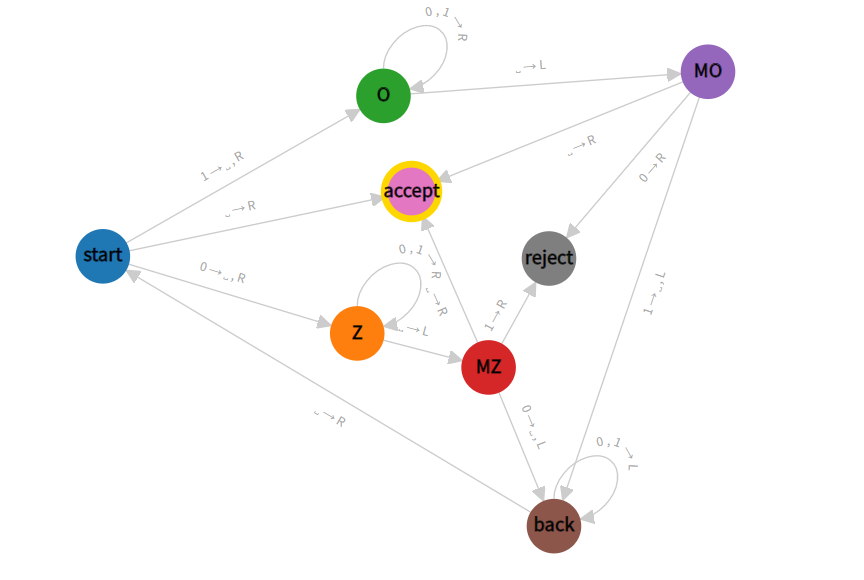
\includegraphics[scale = 0.7]{"C:/Users/Micha/OneDrive - Rensselaer Polytechnic Institute/CSCI 2200/Latex_pictures/Palimdrome_TM.png"}\\
	\end{figure}
\end{center}

%Q (1.32) ends here

\clearpage
\noindent \text{\bf Problem 26.6}. In each case, give high level pseudocode for a Turing Machine M for the problem. Exponential: $L = \{0^{•n}\#1^{•2^n}, n \geq 0\}$ (\# is punctuation).\\\\
Step1: check Input Format:$0^i \# 1^j$\\
Step2: Go back to $*$\\
Step3: Move right come to first unmarked 0, mark it. Go to step 4.

If come to \#, go to Step 7.\\
Step4:Move right to first unmarked 1, mark it.

Move one bit right again. If it is not one, go to REJECT. Else mark it.

If there is no unmarked 1, then go to step 6.

Else Go to step 2.\\
Step 6: Go back to $*$. Move right until you see a \# then ACCEPT. If you see a unmarked 0 then REJECT.\\
Step 7: Go back to $*$. Move right until you see a unmarked 1 then REJECT(Don't reject \#). Else ACCEPT. 


\clearpage

%Q (2.21) starts from here%
\noindent \text{\bf Problem 27.4}. Given an untimate-debugger that determines if a program halts, show how to resolve each conjecture.
(b) The twin primes conjecture that n and n + 2 are prime for infinitely many n.

n = 1\\
While (True):

	if (There does not exist a twin prime number greater than or equal to n):
	
		\qquad break
		
	n = n+1\\
If the Ultimate Debugger says the program halts, then the Conjecture is wrong. If the Ultimate Debugger says the program does not halt, then the Conjecture is right.
\clearpage
\text{\bf Problem 27.48}. Prove that there exists an undecidable language which is a subset of $\{1\}^*$.\\

We can set up a mapping from $\{0,1\}^*$ to $\{1\}^*$ by mapping $x \in \{0,1\}^*$ to $\{1\}^{binx}$ and it is an undecidable set.

\clearpage

%Q (2.26) starts from here
\text{\bf Problem 27.45}. Find a solution to these instances of PCP
\begin{center}
	\begin{figure}[h]
		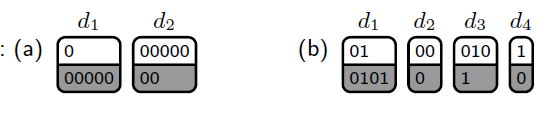
\includegraphics[scale = 0.7]{"C:/Users/Micha/OneDrive - Rensselaer Polytechnic Institute/CSCI 2200/Latex_pictures/27-45.png"}\\
	\end{figure}
\end{center}
(a). d1d1d1d2d2d2d2. In this case we have $3 \times 1 + 5 \times 4 = 23$ 0s on the top row and $5 \times 3 + 4 \times 2 = 23$ 0s on the bottom row. Thus they are equal.\\
(b). d1d1d3d4d4d2d2. The top row is $0101010110000$ and the bottom row is $0101010110000$. Thus they are equal.
%Q (2.26) ends here
\end{document}